%QUESTÃO - Cód.: TF1p0q01

\question [\questaopt] Um pescador encontrou um tesouro e o enterrou 
em um terreno cercado de sua propriedade. Para que ficasse fácil localizar 
o tesouro a qualquer momento, ele fez um esboço do terreno, associando
a ele um sistema de eixos cartesianos. Assim, ele mediu e marcou os
valores indicados na figura.

\begin{center}
	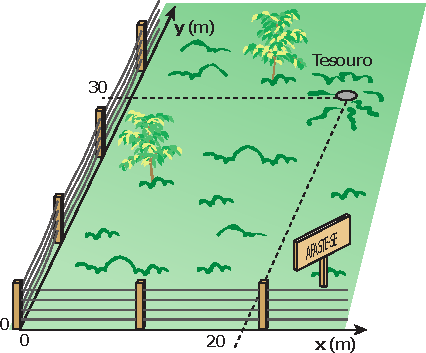
\includegraphics[width=0.4\linewidth]{questoes/imagens/TF1p01q01}
\end{center}



\begin{parts}

	\part Qual a abscissa do local em que está enterrado o tesouro?
	\part Qual a ordenada do local em que está enterrado o tesouro?

\end{parts}


%--------------------------SOLUÇÃO---------------------------------------

	\begin{solution}
		
	(a) 20 m; \\
	(b) 30 m.
		
	\end{solution}

